\noindent

\includegraphics[height=1.25cm]{images/pictograms/benchmark}

\includegraphics[height=1.25cm]{images/pictograms/FEM}

\includegraphics[height=1.25cm]{images/pictograms/wave}

%%%%%%%%%%%%%%%%%%%%%%%%%%%%%%%%%%%%%%%%%%%%%%%%%%%%%%%%%%%%%%%%%%%%%%%%%%%%%%%%%%%%%%%%%%%%%%%%%%%

\begin{flushright} {\tiny {\color{gray} python\_codes/fieldstone\_164/text.tex}} \end{flushright}

%\lstinputlisting[language=bash,basicstyle=\small]{python_codes/template_keywords.key}

\par\noindent\rule{\textwidth}{0.4pt}

\begin{center}
\inpython
{\small Code: \url{https://github.com/cedrict/fieldstone/tree/master/python_codes/fieldstone_164}}
\end{center}

\par\noindent\rule{\textwidth}{0.4pt}

{\sl This stone was developed in collaboration with Donald Duck}. \index{contributors}{D. Duck}

\par\noindent\rule{\textwidth}{0.4pt}

%%%%%%%%%%%%%%%%%%%%%%%%%%%%%%%%%%%%%%%%%%%%%%%%%%%%%%%%%%%%%%%%%%%%%%%%%%%%%%%%%%%%%%%%%%%%%%%%%%%

This \stone solves the 1d wave equation using 1st order finite elements. 
The theory is presented in Chapter~\ref{fem_waveq}. 
This code implements all three methods dealing with the second-order time derivative. 
I recall these here briefly.
We start from the following equation
\[
\M \cdot \vec{\ddot{{\cal U}}}(t) + c^2 \K \cdot \vec{\cal U}(t) = \vec{0}
\]

\begin{itemize}
\item method \# 1
\[
\M \cdot  \vec{\cal U}(t+dt)
= [2  \M  - c^2 dt^2 \K  ]  \cdot \vec{\cal U}(t) - \M \cdot \vec{\cal U}(t-dt)
\]

\item method \# 2 
\[
\M \cdot \vec{\cal W}= -c^2 \K \cdot \vec{\cal U}(t)
\]
\[
\vec{\cal U}(t+dt) = dt^2 \; \vec{\cal W} +2 \vec{\cal U}(t) - \vec{\cal U}(t-dt)
\]

\item method \# 3 
\end{itemize}

At this stage we notice that the FE matrix is simply the 
mass matrix for all three methods. 




The problem at hand is described in Section~\ref{ss:sw1d}.
As such we first create two functions:

\begin{lstlisting}
def u_th(x,t):
    return np.cos(2*np.pi*t)*np.sin(2*np.pi*x)

def udot_th(x,t):
    return -2*np.pi*np.sin(2*np.pi*t)*np.sin(2*np.pi*x)
\end{lstlisting}

The mesh is built simply
\begin{lstlisting}
x=np.linspace(0,Lx,nnx)
\end{lstlisting}
The connectivity array is also very simple in 1d:
\begin{lstlisting}
icon=np.zeros((m,nelx),dtype=np.int32)
for iel in range(0,nelx):
    icon[0,iel]=iel
    icon[1,iel]=iel+1
\end{lstlisting}
where $m$ is the number of nodes per element and $nelx$ the number of elements.

Depending on the metod we will need some or all of these arrays:
$\vec{\cal U}(t)$, $\vec{\cal U}(t-dt)$, $\vec{\cal U}(t+dt)$, $\vec{\dot{{\cal U}}}(t)$, $\vec{\dot{{\cal U}}}(t+dt)$.
All these are $nnx=nelx+1$ long. 
In the code we declare and initialise them as follows 
\begin{lstlisting}
u=np.zeros(nnx,dtype=np.float64)    
uprevprev=np.zeros(nnx,dtype=np.float64) 
uprev=np.zeros(nnx,dtype=np.float64)    
udot=np.zeros(nnx,dtype=np.float64)    
udotprev=np.zeros(nnx,dtype=np.float64) 
for i in range(0,nnx):
    uprevprev[i]=u_th(x[i],0)
    uprev[i]=u_th(x[i],0)+dt*udot_th(x[i],0)
    udotprev[i]=udot_th(x[i],0)
\end{lstlisting}




As shown in Section XXX the mass matrix $\M$ and Laplace matrix $\K$ are 
easily analytically computed for linear 1D elements:
\[
\M_e=
h_x\frac{1}{3}
\left(
\begin{array}{cc}
1 & 1/2 \\ 1/2 & 1
\end{array}
\right)
=
\left(
\begin{array}{cc}
h_x/3 & h_x/6 \\ h_x/6 & h_x/3
\end{array}
\right)
\qquad
\K_e=
\frac{1}{h_x}
\left(
\begin{array}{cc}
1 & -1 \\ -1 & 1
\end{array}
\right)
\]
This translates as follows in the code:
\begin{lstlisting}
Me=np.array([[hx/3,hx/6],[hx/6,hx/3]],dtype=np.float64)
Ke=np.array([[1/hx,-1/hx],[-1/hx,1/hx]],dtype=np.float64)
\end{lstlisting}

In the case we have three elements, the first elemental matrix $\M_e$
gets modify by the application of the boundary conditions:
\begin{verbatim}
[[0.11111111 0.        ]
 [0.         0.11111111]]
\end{verbatim}
The second elemental matrix is simply $\M_e$
\begin{verbatim}
[[0.11111111 0.05555556]
 [0.05555556 0.11111111]]
\end{verbatim}
and the third elemental matrix is also modified bc of boundary conditions:
\begin{verbatim}
[[0.11111111 0.        ]
 [0.         0.11111111]]
\end{verbatim}
When assembled we obtain the following FE matrix:
\begin{verbatim}
[[0.11111111 0.         0.         0.        ]
 [0.         0.22222222 0.05555556 0.        ]
 [0.         0.05555556 0.22222222 0.        ]
 [0.         0.         0.         0.11111111]]
\end{verbatim}



%=====================================================
\section*{Results}


The following results are obtained for $nelx=20$ with all three methods.
The time step is set to $dt=10^{-3}$. 

\begin{center}
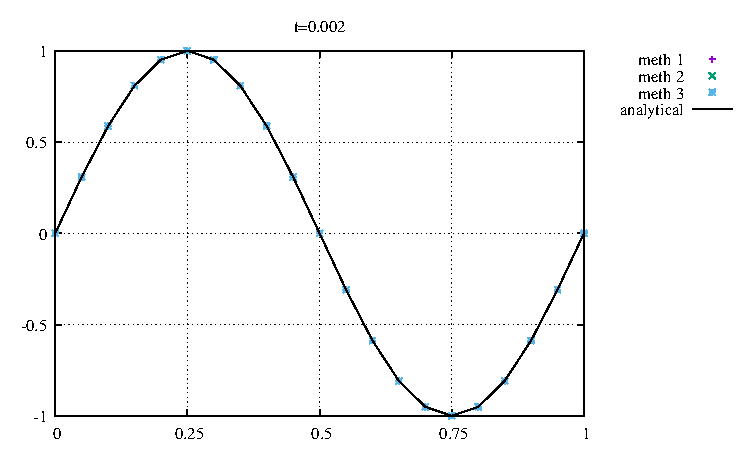
\includegraphics[width=8cm]{python_codes/fieldstone_164/results/u_0.pdf}
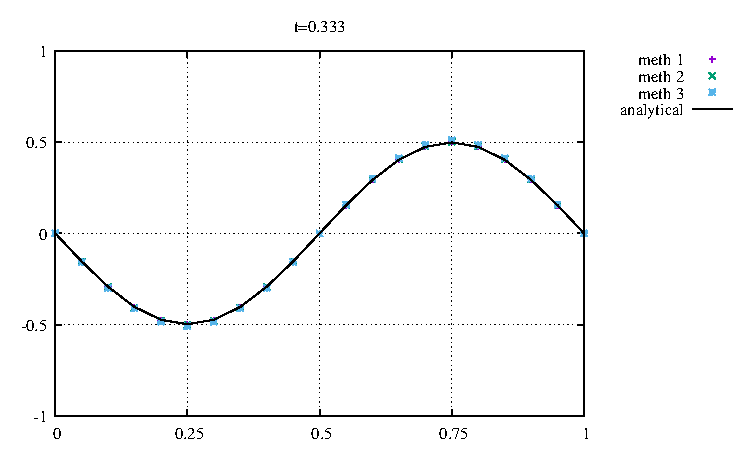
\includegraphics[width=8cm]{python_codes/fieldstone_164/results/u_1.pdf}\\
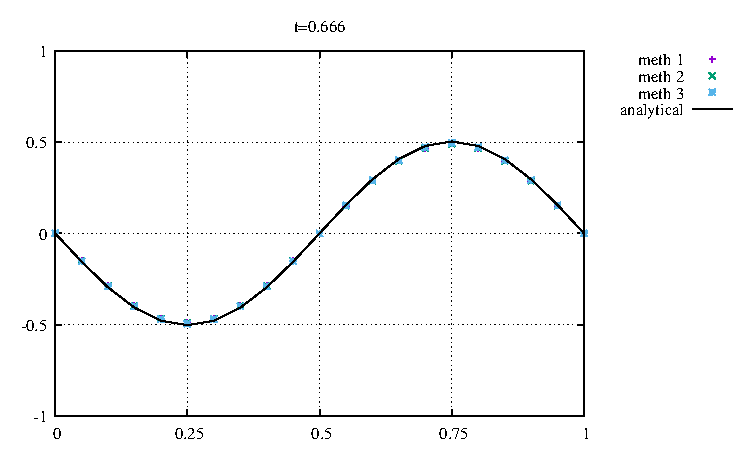
\includegraphics[width=8cm]{python_codes/fieldstone_164/results/u_2.pdf}
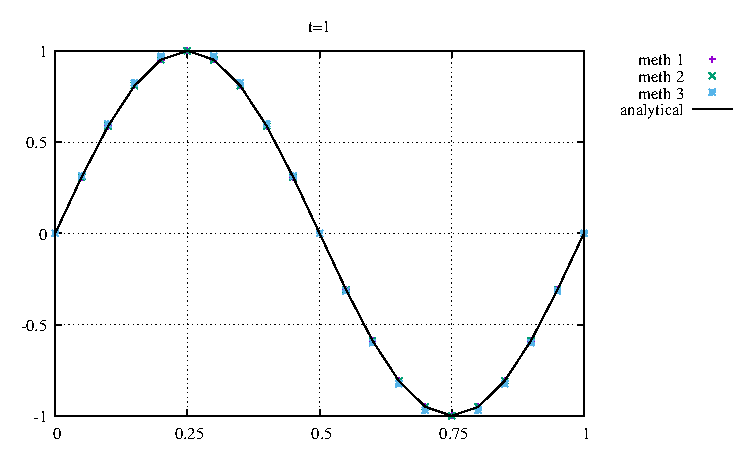
\includegraphics[width=8cm]{python_codes/fieldstone_164/results/u_3.pdf}\\
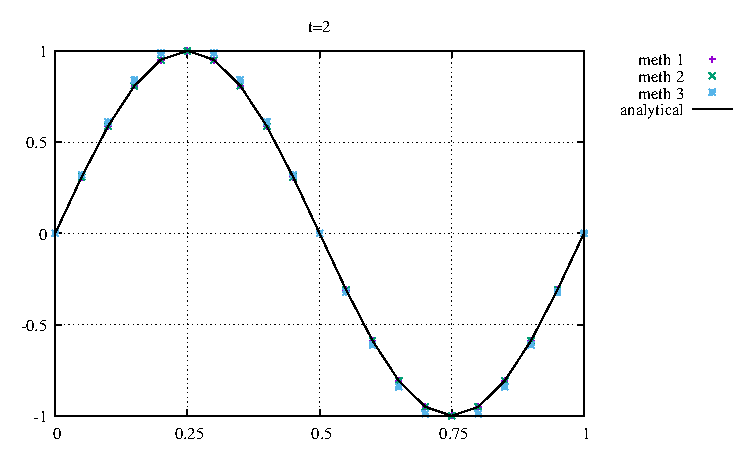
\includegraphics[width=8cm]{python_codes/fieldstone_164/results/u_4.pdf}
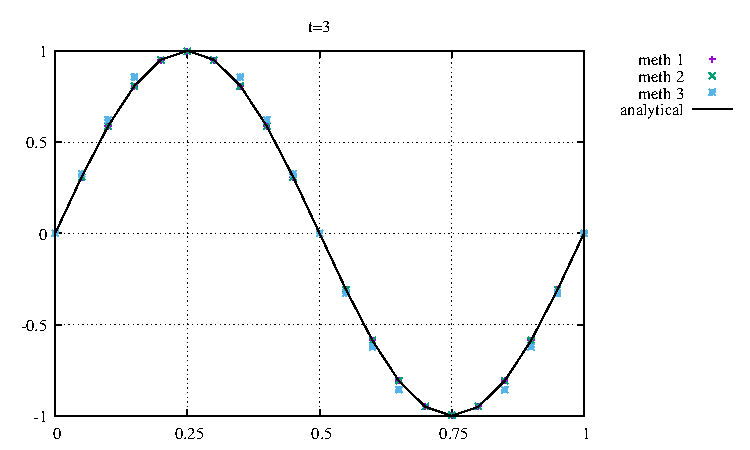
\includegraphics[width=8cm]{python_codes/fieldstone_164/results/u_5.pdf}\\
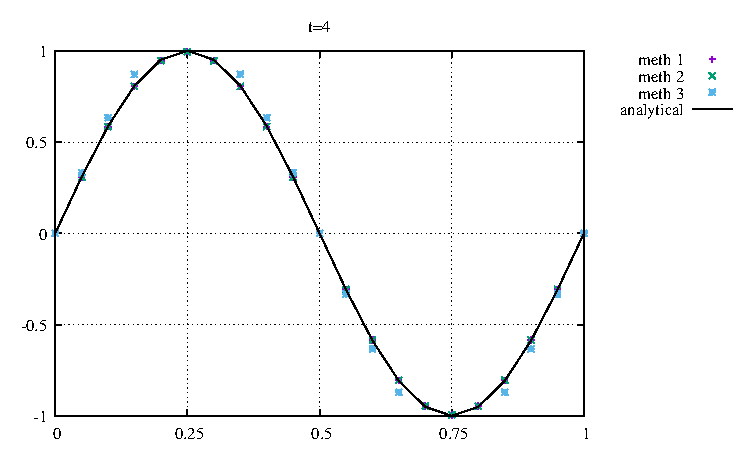
\includegraphics[width=8cm]{python_codes/fieldstone_164/results/u_6.pdf}
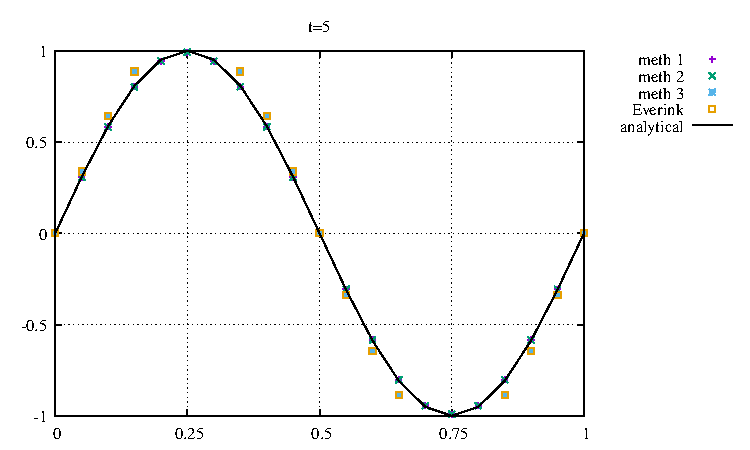
\includegraphics[width=8cm]{python_codes/fieldstone_164/results/u_7.pdf}
\end{center}

I need to plot everunk's data against mine!

